\documentclass[conference]{IEEEtran}
\IEEEoverridecommandlockouts

\usepackage{cite}
\usepackage{amsmath,amssymb}
\usepackage{graphicx}
\usepackage{booktabs}
\usepackage{array}
\usepackage[table]{xcolor}
\usepackage{tikz}
\usetikzlibrary{positioning,arrows.meta}
\usepackage[caption=false,font=footnotesize]{subfig}
\usepackage[hyphens]{url}
\usepackage[hidelinks]{hyperref}
\hypersetup{
  pdftitle={From Audit to Accountability: An Algorithmic Impact Assessment and Regulatory Review of Cost-as-a-Proxy Healthcare Algorithms},
  pdfauthor={Aditya Ravi, Aayush Tiwari, Atharva Indulkar},
  pdfsubject={Ethics of AI and data science},
  pdfkeywords={algorithmic fairness, healthcare, label bias, impact assessment, accountability, AI regulation}
}

% Generated by analysis/tables.py
\newcommand{\NPatients}{48{,}784}
\newcommand{\NBlack}{5{,}582}
\newcommand{\ShareBlack}{11.4\%}
\newcommand{\NTrain}{29{,}270}
\newcommand{\NHoldout}{19{,}514}
\newcommand{\NFeatures}{149}
\newcommand{\GapHealth}{0.61}
\newcommand{\GapHealthLo}{0.56}
\newcommand{\GapHealthHi}{0.67}
\newcommand{\GapHealthRel}{45\%}
\newcommand{\GapCost}{$+$\$298}
\newcommand{\GapCostLo}{$-$\$221}
\newcommand{\GapCostHi}{$+$\$838}
\newcommand{\TopShareBlack}{20.0\%}
\newcommand{\TopShareBlackLo}{18.1\%}
\newcommand{\TopShareBlackHi}{21.9\%}
\newcommand{\TopCondB}{6.62}
\newcommand{\TopCondW}{5.21}
\newcommand{\TopCondRel}{27\%}
\newcommand{\CostEqualHealth}{$-$\$734}
\newcommand{\CostEqualHealthLo}{$-$\$1{,}347}
\newcommand{\CostEqualHealthHi}{$-$\$161}
\newcommand{\AvoidGap}{$-$\$287}
\newcommand{\BlackLeFive}{91\%}
\newcommand{\SwapBefore}{18.4\%}
\newcommand{\SwapBuggy}{44.8\%}
\newcommand{\SwapFixed}{59.2\%}
\newcommand{\SwapOracle}{23.7\%}
\newcommand{\SwapN}{1{,}950}
\newcommand{\NEnrolled}{452}
\newcommand{\EnrolGap}{0.6}
\newcommand{\EnrolGapLo}{$-$0.1}
\newcommand{\EnrolGapHi}{1.2}
\newcommand{\EnrolCondB}{5.66}
\newcommand{\EnrolCondW}{4.42}
\newcommand{\EnrolCondGap}{1.24}
\newcommand{\EnrolCondGapLo}{0.49}
\newcommand{\EnrolCondGapHi}{2.12}
\newcommand{\LabCost}{19.0\%}
\newcommand{\LabAvoid}{25.8\%}
\newcommand{\LabHealth}{28.2\%}
\newcommand{\LabCommercial}{20.0\%}
\newcommand{\ExcessHealth}{94\%}
\newcommand{\ExcessAvoid}{53\%}
\newcommand{\BlendBlack}{25.5\%}
\newcommand{\BlendCost}{16.8\%}
\newcommand{\BlendExcess}{46\%}
\newcommand{\CostOnlyCost}{16.8\%}
\newcommand{\CostOnlyBlack}{19.0\%}
\newcommand{\BlendRho}{0.989}
\newcommand{\RepRatio}{0.80}
\newcommand{\NeedShare}{25.0\%}
\newcommand{\PpvB}{47\%}
\newcommand{\PpvW}{33\%}


% Status marks used in the regulatory and AIA tables
\DeclareRobustCommand{\mY}{\tikz[baseline=-0.6ex]\fill[black] (0,0) rectangle (1.7mm,1.7mm);}
\DeclareRobustCommand{\mP}{\tikz[baseline=-0.6ex]{\fill[black] (0,0) -- (1.7mm,1.7mm) -- (0,1.7mm) -- cycle;\draw[line width=0.4pt] (0,0) rectangle (1.7mm,1.7mm);}}
\DeclareRobustCommand{\mN}{\tikz[baseline=-0.6ex]\draw[line width=0.4pt] (0,0) rectangle (1.7mm,1.7mm);}
\DeclareRobustCommand{\mX}{\tikz[baseline=-0.6ex]{\draw[line width=0.4pt,red!70!black] (0,0) rectangle (1.7mm,1.7mm);\draw[line width=0.4pt,red!70!black] (0,0) -- (1.7mm,1.7mm) (0,0.85mm) -- (0.85mm,1.7mm) (0.85mm,0) -- (1.7mm,0.85mm);}}

% A row break inside the IEEEtran author block (for the repository link)
\makeatletter
\newcommand{\linebreakand}{%
  \end{@IEEEauthorhalign}
  \hfill\mbox{}\par
  \mbox{}\hfill\begin{@IEEEauthorhalign}
}
\makeatother

\newcommand{\repo}{\href{https://github.com/aditya-ravi11/EAIDS}{\texttt{github.com/aditya-ravi11/EAIDS}}}
\newcommand{\site}{\href{https://aditya-ravi11.github.io/EAIDS/}{\texttt{aditya-ravi11.github.io/EAIDS}}}

\begin{document}

\title{From Audit to Accountability: An Algorithmic Impact Assessment and Regulatory Review of Cost-as-a-Proxy Healthcare Algorithms}

\author{
\IEEEauthorblockN{Aditya Ravi}
\IEEEauthorblockA{Roll No.\ 16014223004\\Batch B2}
\and
\IEEEauthorblockN{Aayush Tiwari}
\IEEEauthorblockA{Roll No.\ 16014223003\\Batch B2}
\and
\IEEEauthorblockN{Atharva Indulkar}
\IEEEauthorblockA{Roll No.\ 16014223022\\Batch B2}
\linebreakand
\IEEEauthorblockA{GitHub repository: \repo}
}

\maketitle

\begin{abstract}
Commercial risk scores decide which patients are enrolled in high-risk care-management programmes, and a widely used class of such tools predicts future \emph{cost} as a proxy for health \emph{need}. Obermeyer et al.\ showed in 2019 that this proxy under-refers Black patients. Detection is no longer the open problem; governance is. We first reproduce the audit on the authors' public synthetic cohort ($n=\NPatients$ patient-years), re-implementing the counterfactual analysis with its 2022 correction and matching the published synthetic outputs to four decimal places. At equal risk scores, Black patients carry \GapHealth{} more active chronic conditions (95\% CI \GapHealthLo--\GapHealthHi), while the score's calibration on cost does not differ by race. Training one model class on three labels shows that the label, not the model, drives the disparity: the Black share of the top 3\% rises from \LabCost{} (cost) to \LabHealth{} (chronic conditions), and a blended label closes \BlendExcess{} of the excess-illness gap while capturing the same share of spending. Human review did not correct the score. We then propose a seven-gate algorithmic impact assessment (AIA) whose decisive gate, a label-validity test, the deployment would have failed, together with an accountability matrix for vendor, hospital, clinicians, payer and regulator. Finally, we code eight obligations across the United States, the European Union and India for 2019 and 2026. As of October 2026, no jurisdiction clearly requires the missing test for this deployment, and US federal protection against race-blind proxy discrimination has narrowed. An interactive dashboard accompanies the paper at \site.
\end{abstract}

\begin{IEEEkeywords}
algorithmic fairness, label bias, healthcare AI, algorithmic impact assessment, accountability, AI regulation, EU AI Act, DPDP Act
\end{IEEEkeywords}

%=====================================================================
\section{Problem Definition}
%=====================================================================
Hospitals and insurers run high-risk care-management programmes that give a small group of patients additional nursing support, priority appointments and closer follow-up. Because places are scarce, patients are ranked by an algorithmic risk score. In the health system studied by Obermeyer et al.~\cite{obermeyer2019}, patients at or above the 97th percentile of a commercial score were automatically identified for enrolment and those above the 55th percentile were flagged to their primary-care physician. By industry estimates, tools of this class are applied to roughly 200 million people in the United States each year~\cite{obermeyer2019}. The paper did not name the product; it was identified in press coverage and in a letter from New York regulators as Optum's Impact Pro~\cite{dfs2019,ledford2019}.

The score was trained to predict next year's total medical expenditure, used as a proxy for health need. Because Black patients in the US receive less care at the same level of illness, through differences in access, insurance, geography and trust, an accurate cost model systematically ranks them as healthier than they are. Race was never an input; the disparity entered through the \emph{choice of label}~\cite{obermeyer2019,jacobs2021}.

The bias is now well documented. This project addresses the governance question that remains open: \emph{what should a deploying hospital have done before using such a score, who is accountable for the harm, what assessment should have been required, and would current US, EU and Indian frameworks mandate it?}

%=====================================================================
\section{Objectives}
%=====================================================================
\begin{enumerate}
\item \textbf{Reproduce the audit} on the public synthetic cohort, including the 2022 code correction, and report fidelity against the published values.
\item \textbf{Isolate the label} by training one model class on three targets with identical features.
\item \textbf{Design the missing assessment}: a pre-deployment AIA with measurable pass criteria.
\item \textbf{Assign accountability} across vendor, hospital, clinicians, payer, patients and regulators.
\item \textbf{Test the law}: code US, EU and Indian obligations for 2019 and 2026 and ask whether each would require that assessment.
\item \textbf{Communicate} the analysis through a reproducible, interactive dashboard.
\end{enumerate}

%=====================================================================
\section{Background and Context}
%=====================================================================
\subsection{How a cost prediction becomes a care decision}
Fig.~\ref{fig:pipeline} traces the decision pipeline. A vendor trains a model on claims data; a hospital or payer licenses it, chooses thresholds, and passes a ranked list to care managers, who make the final enrolment decision. Every hand-off is an opportunity to ask what the score measures, and in 2019 no actor in the chain was obliged to ask.

\begin{figure}[t]
\centering
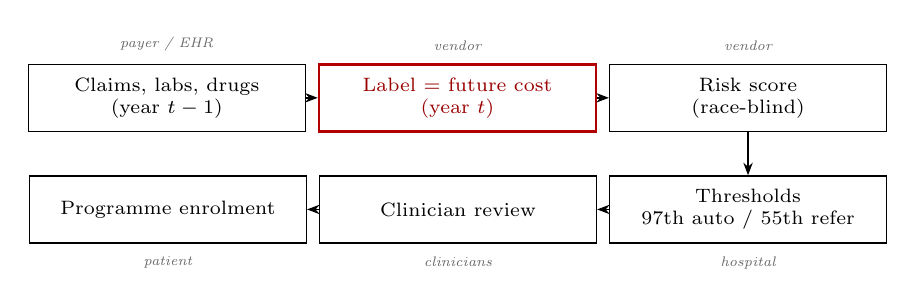
\begin{tikzpicture}[
  node distance=1.5mm,
  box/.style={draw, line width=0.5pt, minimum width=0.29\columnwidth, minimum height=8.5mm, align=center, font=\scriptsize, inner sep=2pt},
  flaw/.style={box, draw=red!70!black, text=red!60!black, line width=0.9pt},
  own/.style={font=\tiny\itshape, text=black!60},
  arr/.style={-{Stealth[length=1.6mm]}, line width=0.5pt}]
\node[box] (a) {Claims, labs, drugs\\(year $t-1$)};
\node[flaw, right=of a] (b) {Label = future cost\\(year $t$)};
\node[box, right=of b] (c) {Risk score\\(race-blind)};
\node[box, below=5.5mm of c] (d) {Thresholds\\97th auto / 55th refer};
\node[box, left=of d] (e) {Clinician review};
\node[box, left=of e] (f) {Programme enrolment};
\draw[arr] (a) -- (b); \draw[arr] (b) -- (c); \draw[arr] (c) -- (d); \draw[arr] (d) -- (e); \draw[arr] (e) -- (f);
\node[own, above=0.4mm of a] {payer / EHR};
\node[own, above=0.4mm of b] {vendor};
\node[own, above=0.4mm of c] {vendor};
\node[own, below=0.4mm of d] {hospital};
\node[own, below=0.4mm of e] {clinicians};
\node[own, below=0.4mm of f] {patient};
\end{tikzpicture}
\caption{Decision pipeline and the actor who controls each step. The design flaw sits with the vendor; the decision to deploy, the thresholds and the outcome sit with the hospital.}
\label{fig:pipeline}
\end{figure}

\subsection{Related work}
Obermeyer et al.~\cite{obermeyer2019} established that the score is calibrated on cost but not on health, and that a label combining health and cost, replicated by the manufacturer on 3,695,943 patients, reduced excess bias by 84\%. Their public release~\cite{labsysmed} includes a synthetic cohort and a 2022 erratum: a bug in the counterfactual ``swap'' understated its result (47\% rather than 59\%), together with Corbett-Davies' observation that the swap is asymmetric. Jacobs and Wallach~\cite{jacobs2021} frame such failures as measurement problems in which the construct (need) and its operationalisation (cost) diverge. Kleinberg et al.~\cite{kleinberg2017} and Chouldechova~\cite{chouldechova2017} prove that common fairness criteria cannot all hold at once, and Corbett-Davies et al.~\cite{corbett2023} argue for judging scores against the decision they serve. On governance, Nissenbaum~\cite{nissenbaum1996} described the ``problem of many hands'', Selbst et al.~\cite{selbst2019} warned against abstracting away the sociotechnical context, and Raji et al.~\cite{raji2020} proposed end-to-end internal audits. Model cards~\cite{mitchell2019} offer a documentation standard. Algorithmic impact assessments were proposed for public agencies by Reisman et al.~\cite{reisman2018}, codified in Canada's Directive on Automated Decision-Making~\cite{canada_dadm}, piloted for healthcare by the Ada Lovelace Institute~\cite{ada2022}, and turned into a practitioner checklist by the Algorithmic Bias Playbook~\cite{booth2021}. Vyas et al.~\cite{vyas2020} show that race-aware clinical algorithms raise related concerns.

\subsection{Regulatory context, 2019--2026}
In 2019, New York's financial and health regulators asked UnitedHealth to show that Impact Pro was not discriminatory or stop using it~\cite{dfs2019}, and US senators wrote to CMS, the FTC and five insurers~\cite{booker2019}. Since then the US adopted a decision-support-tool rule under Section 1557 of the ACA~\cite{hhs1557,ocr2025} and algorithm-transparency rules for certified health IT~\cite{hti1}, but later revoked the federal AI executive order~\cite{eo14148}, deprioritised disparate-impact enforcement~\cite{eo14281,hhs_tvi2026} and moved against state AI laws~\cite{eo14365}. Colorado's AI Act was replaced before taking effect~\cite{colorado}. The EU adopted the AI Act~\cite{euaiact} and then delayed its high-risk obligations through the Digital Omnibus~\cite{omnibus2026}. India enacted the DPDP Act~\cite{dpdp2023} and notified its Rules~\cite{dpdprules2025}, while AI-specific guidance remains voluntary~\cite{icmr2023,niti2021,meity2025}.

%=====================================================================
\section{Ethical Issue Identification}
%=====================================================================
We separate harms arising in \emph{design}, \emph{deployment} and \emph{governance}.

\textbf{E1 Proxy-label bias} (design). Future cost is a biased measurement of future need; an accurate cost model is an inaccurate need model.
\textbf{E2 Fairness through unawareness fails} (design). Excluding race from the inputs was treated as a safeguard, but the disparity entered through the label, and the exclusion also stopped anyone measuring it.
\textbf{E3 Structural inequity encoded} (design, deployment). Historical under-treatment lowers predicted risk, which lowers future care: a feedback loop.
\textbf{E4 Opacity} (governance). The score was proprietary; deployers lacked subgroup performance and patients were not told they had been ranked.
\textbf{E5 Automation bias and thin oversight} (deployment). Clinician review existed but, as shown in Section~\ref{sec:human}, did not correct the disparity.
\textbf{E6 The problem of many hands} (governance). Vendor, payer, hospital and clinicians each controlled one link, so no one owned the outcome~\cite{nissenbaum1996}.
\textbf{E7 No assessment or monitoring} (governance). Nothing required a pre-deployment check, and the bias was found by outside academics rather than by any internal audit or regulator.
\textbf{E8 Scale} (governance). A single design choice replicated across a product class turns a modelling shortcut into a population-level allocation decision.

%=====================================================================
\section{Methodology and Analysis}
\label{sec:method}
%=====================================================================
\subsection{Data}
We use the synthetic cohort released with the original study~\cite{labsysmed}: \NPatients{} patient-years (\NBlack{} Black, \ShareBlack), generated with \emph{synthpop} to mirror the real data's joint distribution. It contains the commercial risk score, programme enrolment, total and avoidable cost, active chronic conditions, five biomarkers, and \NFeatures{} year-$(t-1)$ features. The synthetic file has no patient identifier and fewer rows than the paper's 100,009, so we report its results alongside the published values (Table~\ref{tab:fidelity}) and do not treat them as real-world magnitudes. The raw file is downloaded by script and never redistributed. All analysis code is in the repository (\repo).

\subsection{Calibration audit}
Risk-score percentiles are computed from ranks (0--99). For outcome $y$ we estimate the within-percentile racial gap $\Delta$ from $y_i=\Delta\,\mathrm{Black}_i+\gamma_{p(i)}+\varepsilon_i$ with percentile fixed effects $\gamma_p$, and report 95\% percentile-bootstrap intervals from 1,000 row resamples (seed 0). Fig.~\ref{fig:calibration} shows the result. On health, $\Delta_H=\GapHealth$ conditions (\GapHealthLo--\GapHealthHi), or \GapHealthRel{} of the mean. On cost, $\Delta_C$ is \GapCost{} (\GapCostLo{} to \GapCostHi), an interval containing zero. The score is fair by the criterion its vendor would check and unfair by the one the programme needs. At or above the 97th percentile, Black patients have \TopCondB{} active chronic conditions against \TopCondW{} for White patients (+\TopCondRel; published: 4.8 vs 3.8, +26\%).

\begin{figure*}[t]
\centering
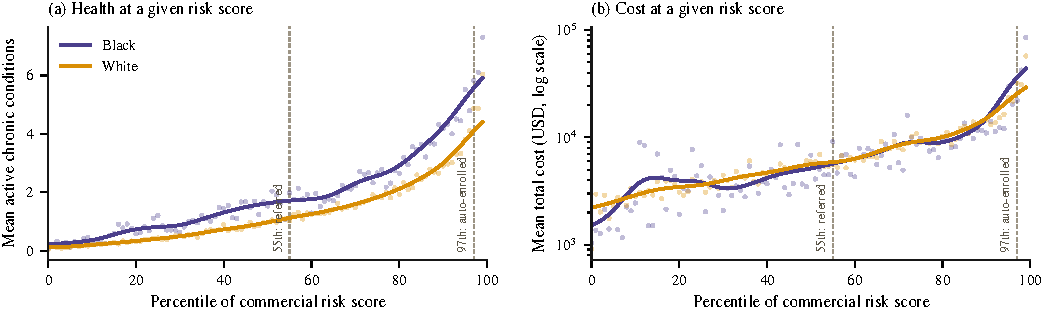
\includegraphics[width=\textwidth]{figures/calibration.pdf}
\caption{Calibration by race. (a) Mean active chronic conditions in year $t$ by percentile of the commercial risk score; (b) mean total cost (log scale). Dots are percentile means; lines are count-weighted Gaussian kernel smooths. Dashed lines mark the programme thresholds.}
\label{fig:calibration}
\end{figure*}

\subsection{Mechanism and biomarkers}
Regressing cost on race with fixed effects for the number of active conditions gives a gap of \CostEqualHealth{} per patient-year (95\% CI \CostEqualHealthLo{} to \CostEqualHealthHi; published $-$\$1{,}801). Black spending is lower at every level up to five conditions, which covers \BlackLeFive{} of Black patient-years (Fig.~\ref{fig:mechanism}); above that the cells are small and the pattern is noisy. Spending is the label, so this gap becomes the bias. The gap in avoidable (emergency and inpatient) cost is smaller (\AvoidGap, interval includes zero), which anticipates why an avoidable-cost label is less biased. Fig.~\ref{fig:biomarkers} repeats the calibration check on biomarkers by score decile. At equal scores, Black patients have higher HbA1c, systolic blood pressure and creatinine and lower hematocrit, indicating worse diabetes, hypertension, kidney function and anaemia. Biomarkers are missing where tests were not ordered, so these comparisons describe the tested population only.

\begin{figure}[t]
\centering
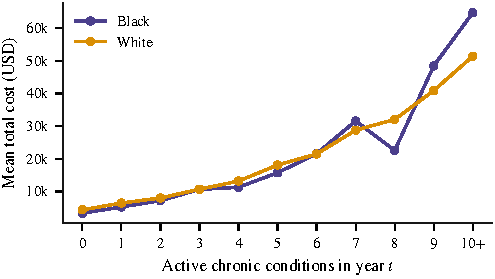
\includegraphics[width=\columnwidth]{figures/mechanism.pdf}
\caption{Mean total cost by number of active chronic conditions. Up to five conditions (\BlackLeFive{} of Black patient-years), less is spent on Black patients at every level; higher levels have few patients.}
\label{fig:mechanism}
\end{figure}

\begin{figure*}[t]
\centering
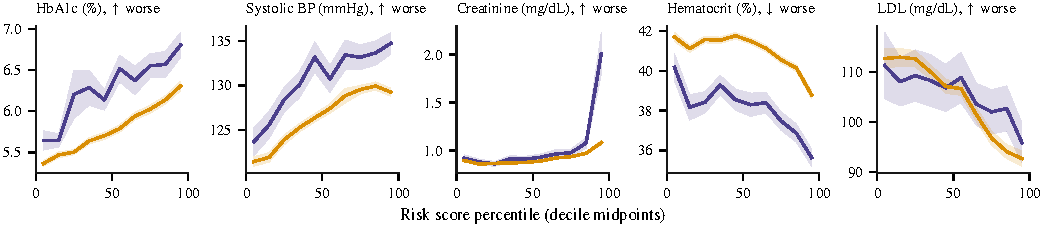
\includegraphics[width=\textwidth]{figures/biomarkers.pdf}
\caption{Biomarkers by risk-score decile with 95\% intervals (indigo: Black; amber: White). At equal scores, Black patients' clinical markers are worse.}
\label{fig:biomarkers}
\end{figure*}

\subsection{Counterfactual swap}
We re-implemented the authors' exercise in Python. Starting from the patients above a threshold, the healthiest enrolled White patient is replaced by the highest-scored Black patient below the threshold whenever the latter has strictly more conditions. Using the authors' percentile binning (top 4\%, $n=\SwapN$), the pre-2022 logic returns \SwapBefore{}$\rightarrow$\SwapBuggy, matching their published synthetic output to four decimal places and serving as a regression test. The corrected logic returns \SwapFixed{}, matching their erratum (Fig.~\ref{fig:swap}). Because the swap only removes White patients and only adds Black ones, we also fill the same number of places purely by realised chronic conditions. That gives \SwapOracle{} Black. The 59\% figure therefore shows how many Black patients below the line are sicker than White patients above it; it is not the composition of an unbiased programme.

\begin{figure}[t]
\centering
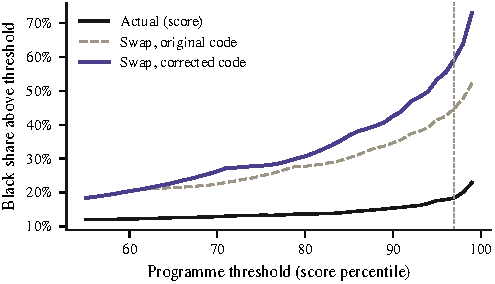
\includegraphics[width=\columnwidth]{figures/swap.pdf}
\caption{Counterfactual swap across thresholds: actual Black share, the original (pre-2022) code and the corrected code.}
\label{fig:swap}
\end{figure}

\subsection{Label-choice experiment}
To separate the label from the model, we train the same estimator on three targets: $\log(1+\text{total cost})$, $\log(1+\text{avoidable cost})$, and active chronic conditions. The estimator is a LASSO pipeline (standardisation, 10-fold cross-validated penalty) on all year-$(t-1)$ claims, laboratory, medication and demographic features, with race excluded. An assertion guards against leakage of year-$t$ variables. The split is a deterministic 60/40 ($n_{\text{train}}=\NTrain$, $n_{\text{hold-out}}=\NHoldout$). We report the Black share of the top 3\%, with a bootstrap interval over the hold-out set conditional on the fitted model, and the share of total cost, avoidable cost and conditions captured. We also report the \emph{excess-conditions} statistic used in the vendor's replication: the sum, over Black patients, of their chronic conditions minus the White mean at the same score percentile. Finally, we trace a frontier of blended scores $s_\alpha=\alpha\,z(\hat{y}_{\text{cost}})+(1-\alpha)\,z(\hat{y}_{\text{health}})$ for $\alpha\in[0,1]$. Retraining directly on the $\alpha=0.5$ label reproduces the blended ranking (Spearman $\rho=\BlendRho$).

\subsection{Selection fairness}
At a programme capacity $k$, we define the \emph{truly high-need} group as the $k$ patients with the most realised chronic conditions, giving tied patients at the cut-off fractional membership. We compare the Black share of selected patients with the Black share of this group (the \emph{representation ratio}), and report precision (PPV) and recall (TPR) by race. Because chronic-condition counts depend on diagnoses being recorded, these estimates are lower bounds. We test sensitivity with two absolute definitions: at least three conditions, and uncontrolled diabetes or hypertension (HbA1c$\geq$9 or systolic BP$\geq$140).

\subsection{Human in the loop}
\label{sec:human}
Enrolment was ultimately a clinician decision (\NEnrolled{} patient-years). Among patients flagged at or above the 55th percentile, Black patients were enrolled at a rate only \EnrolGap{} percentage points higher at the same score percentile (95\% CI \EnrolGapLo{} to \EnrolGapHi). Enrolled Black patients still had \EnrolCondB{} chronic conditions against \EnrolCondW{} for enrolled White patients (difference \EnrolCondGap, CI \EnrolCondGapLo--\EnrolCondGapHi). Human review was present but did not remove the higher bar.

\subsection{Regulatory coding}
For each jurisdiction we coded eight obligations a hospital deploying this score could face, at three dates: October 2019, October 2026, and December 2027 as scheduled. A cell is \mY{} if a binding duty applies to \emph{this} deployment, a race-blind cost-trained enrolment score used by a hospital. It is \mP{} if a binding duty is narrow, not triggered, or adopted but not yet applicable. It is \mN{} if there is no binding duty (soft law counts as \mN), and \mX{} if a 2019 protection has been removed. Every cell was checked against primary sources (Federal Register, EUR-Lex, the Gazette of India and agency documents) as of 7 October 2026.

\subsection{Dashboard}
All numbers, figures and tables are generated by one pipeline (\texttt{analysis/run\_all.py}) and written as JSON. The same JSON drives an interactive static website (Vite and TypeScript, D3 scales) deployed at \site{} and the generated \LaTeX{} tables in this paper.

%=====================================================================
\section{Relevant Ethical Principles}
%=====================================================================
Table~\ref{tab:principles} maps the breached principles onto the frameworks a hospital in each jurisdiction would cite. In principlist terms~\cite{beauchamp2019}, the primary breach is of \emph{justice}: patients with equal need had unequal access to a beneficial programme. The secondary breaches are of \emph{non-maleficence} and \emph{beneficence}, since preventive care was withheld from sicker patients. WHO's guidance~\cite{who2021} names inclusiveness and equity and responsibility and accountability; India's ICMR guidelines~\cite{icmr2023} list non-discrimination and fairness, accountability and liability, and \emph{validity}, the principle most directly violated by an untested proxy. NITI Aayog~\cite{niti2021} and MeitY~\cite{meity2025} add equality and ``understandable by design''. NIST's AI RMF~\cite{nist2023} requires systems to be valid and reliable and ``fair, with harmful bias managed''; the EU HLEG~\cite{hleg2019} adds human agency and oversight. The frameworks disagree on vocabulary but not on substance: every one names fairness, accountability and validity, and this case breaches all three. Privacy creates a real tension, because detecting the bias requires processing race data that data-protection law restricts.

\begin{table*}[t]
\centering
\caption{Crosswalk of the principles breached onto health- and AI-ethics frameworks~\cite{who2021,icmr2023,meity2025,nist2023}.}
\label{tab:principles}
\footnotesize
\renewcommand{\arraystretch}{1.12}
\begin{tabular}{@{}>{\raggedright\arraybackslash}p{3.1cm} >{\raggedright\arraybackslash}p{3.4cm} >{\raggedright\arraybackslash}p{3.6cm} >{\raggedright\arraybackslash}p{2.9cm} >{\raggedright\arraybackslash}p{3.2cm}@{}}
\toprule
Principle & WHO 2021 & ICMR 2023 & MeitY 2025 & NIST AI RMF \\
\midrule
Justice \& non-discrimination & Ensure inclusiveness and equity & Non-discrimination and fairness; accessibility, equity and inclusiveness & Fairness \& equity & Fair, with harmful bias managed \\
Beneficence \& non-maleficence & Promote human well-being, safety and the public interest & Safety and risk minimisation & Safety, resilience \& sustainability & Safe \\
Validity of what is measured & Well-being: accuracy and efficacy in intended use & Validity; optimisation of data quality & Safety, resilience \& sustainability & Valid and reliable \\
Transparency \& explicability & Ensure transparency, explainability and intelligibility & Trustworthiness & Understandable by design & Explainable and interpretable \\
Accountability \& responsibility & Foster responsibility and accountability & Accountability and liability & Accountability & Accountable and transparent \\
Autonomy \& human oversight & Protect human autonomy & Autonomy & People first & — (GOVERN: human--AI roles) \\
Privacy \& data governance & Protect autonomy: privacy and confidentiality & Data privacy & Trust is the foundation & Privacy-enhanced \\
\bottomrule
\end{tabular}
\end{table*}


%=====================================================================
\section{Proposed Solution and Recommendations}
%=====================================================================
\subsection{A seven-gate algorithmic impact assessment}
We propose a pre-deployment AIA for population-health risk tools (Table~\ref{tab:aia}). It combines Canada's impact levels~\cite{canada_dadm}, the participatory stages of the Ada Lovelace pilot~\cite{ada2022}, the Bias Playbook~\cite{booth2021} and NIST's Govern--Map--Measure--Manage cycle~\cite{nist2023}. A tool that rations access to care for large numbers of patients, with effects that are hard to reverse, is Level~III--IV. That level triggers peer review, publication and human decision-making. The decisive addition is \textbf{G1, label validity}: plot need against the score by group before use, and fail the tool if, in the selection band, the upper 95\% bound of the need gap exceeds 0.25 conditions or the relative gap exceeds 5\%. These thresholds are our proposal and should be justified locally. The test needs only data a hospital already holds. G2 then compares selection with a capacity-matched need group (pass if the representation ratio is at least 0.9 for every group and the precision gap is under 10 points). G3 covers rights and stakeholders, G4 mitigation and oversight, G5 a signed and published go/no-go decision, and G6 monitoring with defined re-assessment triggers.

\begin{table*}[t]
\centering
\caption{Proposed seven-gate algorithmic impact assessment (AIA) and the retrospective verdict for the deployment studied. G1 is decisive.}
\label{tab:aia}
\renewcommand{\arraystretch}{1.15}
\begin{tabular}{@{}l >{\raggedright\arraybackslash}p{3.3cm} >{\raggedright\arraybackslash}p{9.6cm} l@{}}
\toprule
Gate & Name & Pass criterion & Retrospective \\
\midrule
G0 & Inventory \& intended use & The label and intended use are written down and match. A mismatch (predicts cost, used for need) is flagged for G1. & \mP\ Partial \\
G1 & \textbf{Label validity} & Upper 95\% bound of the need gap in the selection band below 0.25 conditions, or relative gap under 5\%. & \mX\ Failed \\
G2 & Disparity testing & Representation ratio of at least 0.9 for every group, and no group held to a visibly higher bar (precision gap under 10 points). & \mN\ Not done \\
G3 & Rights \& stakeholder review & Panel held, impact level assigned, and its requirements adopted (Level III--IV for this tool). & \mN\ Not done \\
G4 & Mitigation \& oversight design & G1 and G2 pass after mitigation; enrolled patients equally sick across groups. & \mP\ Partial \\
G5 & Go / no-go \& publication & Named accountable owner; summary published before launch. & \mN\ Not done \\
G6 & Monitoring \& re-assessment & G1--G2 re-run at least annually and on every trigger; results reported to the governance committee. & \mN\ Not done \\
\bottomrule
\end{tabular}
\end{table*}


\subsection{Accountability}
Accountability follows \emph{use} (Table~\ref{tab:raci}). The vendor is responsible for the label and for disclosing what it measures, with subgroup calibration on need as well as cost. The deploying hospital's AI governance body is accountable for the outcome: it chooses to deploy, sets thresholds and answers to patients and regulators. Where a payer licenses or mandates the tool, it shares that accountability. Clinicians are responsible for enrolment decisions, and those decisions must themselves be audited by group. Regulators are accountable for the legal floor. Each activity has exactly one accountable party, which closes the many-hands gap (E6).

\begin{table}[t]
\centering
\caption{Accountability matrix (R responsible, A accountable, C consulted, I informed). Gov.: hospital AI governance; DS: hospital data science; Clin.: clinicians; Eq.: equity officer; Pat.: patients.}
\label{tab:raci}
\scriptsize
\setlength{\tabcolsep}{1.6pt}
\begin{tabular}{@{}lcccccccc@{}}
\toprule
Activity & Vend. & Gov. & DS & Clin. & Eq. & Payer & Pat. & Reg. \\
\midrule
Choose the model's label & \textbf{A/R} & C & C & I & C & C & I & I \\
Disclose label \& subgroup performance & \textbf{A/R} & I & C & I & I & I & I & I \\
Local label-validity \& bias audit (G1--G2) & C & \textbf{A} & R & C & R & I & I & I \\
Set threshold \& capacity & C & \textbf{A} & R & C & C & C & I & I \\
Approve deployment (G5) & I & \textbf{A/R} & C & C & C & I & C & I \\
Review \& override referrals & I & \textbf{A} & I & R & C & I & I & I \\
Monitor \& report incidents (G6) & C & \textbf{A} & R & R & C & I & I & I \\
Retrain or replace the model & R & \textbf{A} & R & I & C & C & I & I \\
Patient notice \& complaints & I & \textbf{A} & I & R & R & I & C & I \\
Set \& enforce the legal floor & I & I & I & I & I & I & C & \textbf{A/R} \\
\bottomrule
\end{tabular}
\end{table}


\subsection{Actions by actor}
\textbf{Vendors:} state the training label prominently; report calibration on need by race, sex and age; offer a blended-label version.
\textbf{Hospitals:} run G0--G6 before go-live and for every new version or threshold; name an accountable executive; publish the AIA summary; collect race and ethnicity data for auditing under strict purpose limitation.
\textbf{Clinicians:} treat the score as a referral aid rather than an eligibility test, record override reasons, and audit enrolment quarterly by group.
\textbf{US regulators:} extend 45~CFR~92.210(b) from tools whose \emph{inputs} measure protected traits to tools whose \emph{labels} can encode protected-trait disparities, and restore an effects-based route for proxy discrimination in federally funded health programmes.
\textbf{EU regulators:} clarify that private providers rationing access to care fall within Annex~III 5(a), or an equivalent FRIA duty, and use the new Article~4a to require, not merely permit, subgroup testing.
\textbf{Indian regulators:} make ICMR's validity and fairness principles binding pre-deployment checks for hospital AI, and designate large health data fiduciaries as Significant Data Fiduciaries so that Rule~13 applies. Public insurers bound by Articles 14--15 can require G1 in procurement today.

%=====================================================================
\section{Results and Findings}
%=====================================================================
\begin{figure*}[!tp]
\centering
\subfloat[Landing view: unit chart of programme places under the cost and health rankings]{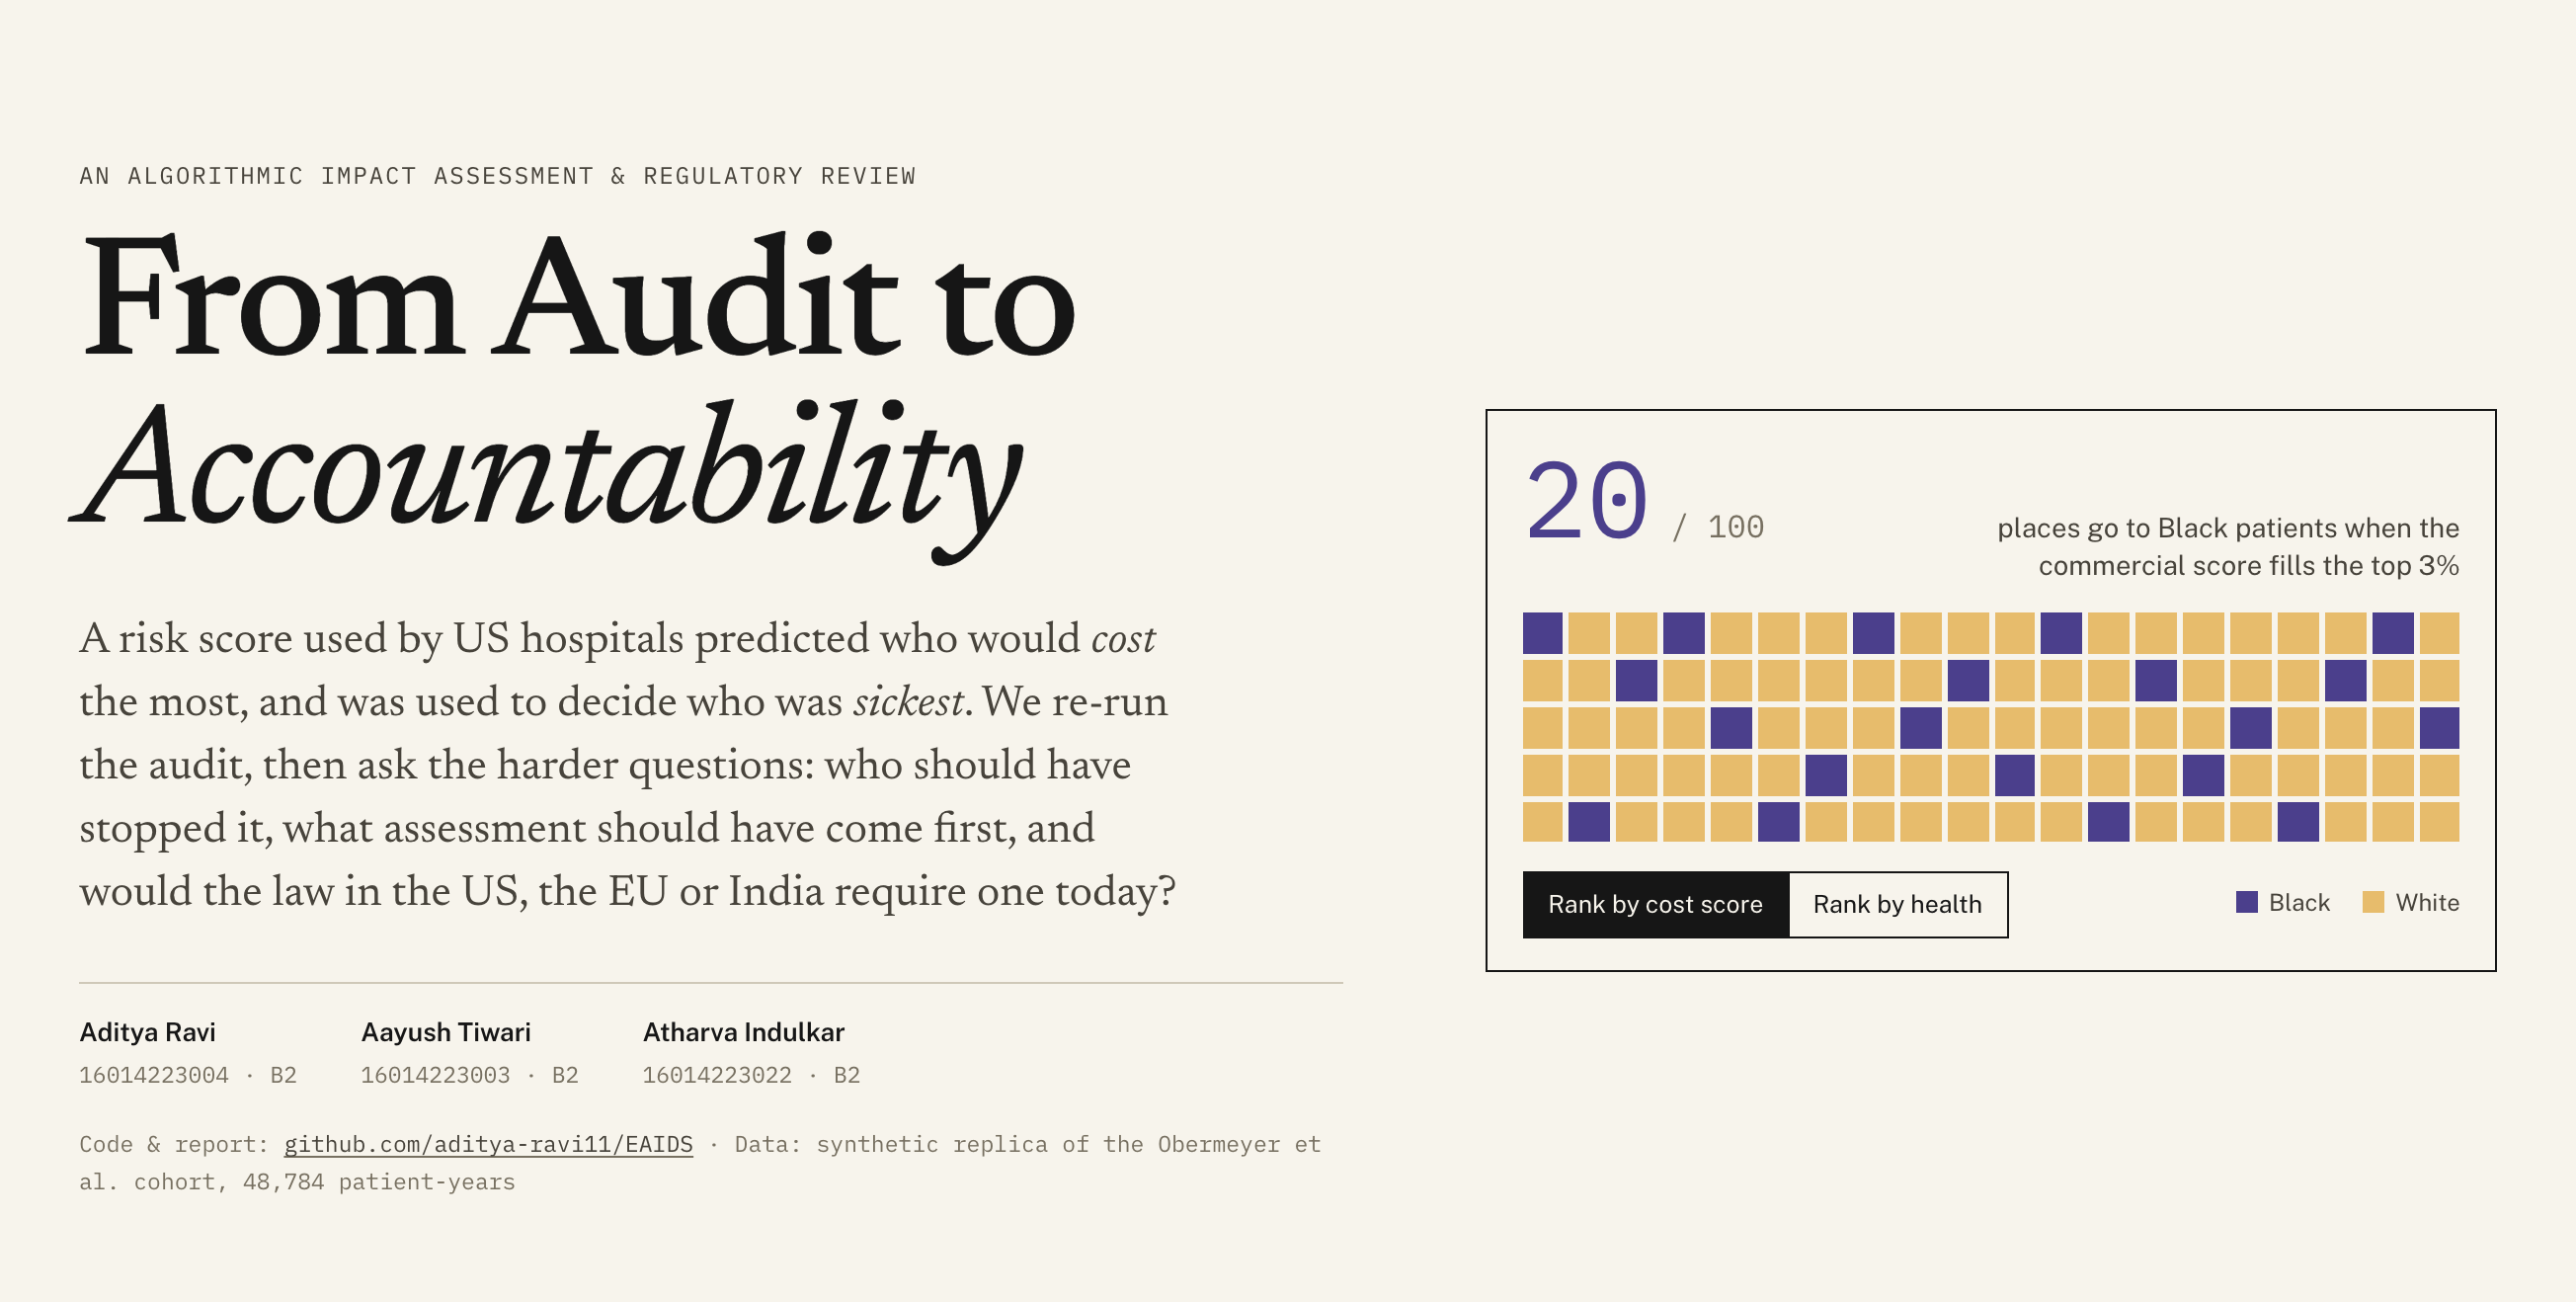
\includegraphics[width=\textwidth]{figures/screens/hero.png}}\\[1mm]
\subfloat[Threshold explorer: Black share selected vs.\ the truly high-need, with live readout]{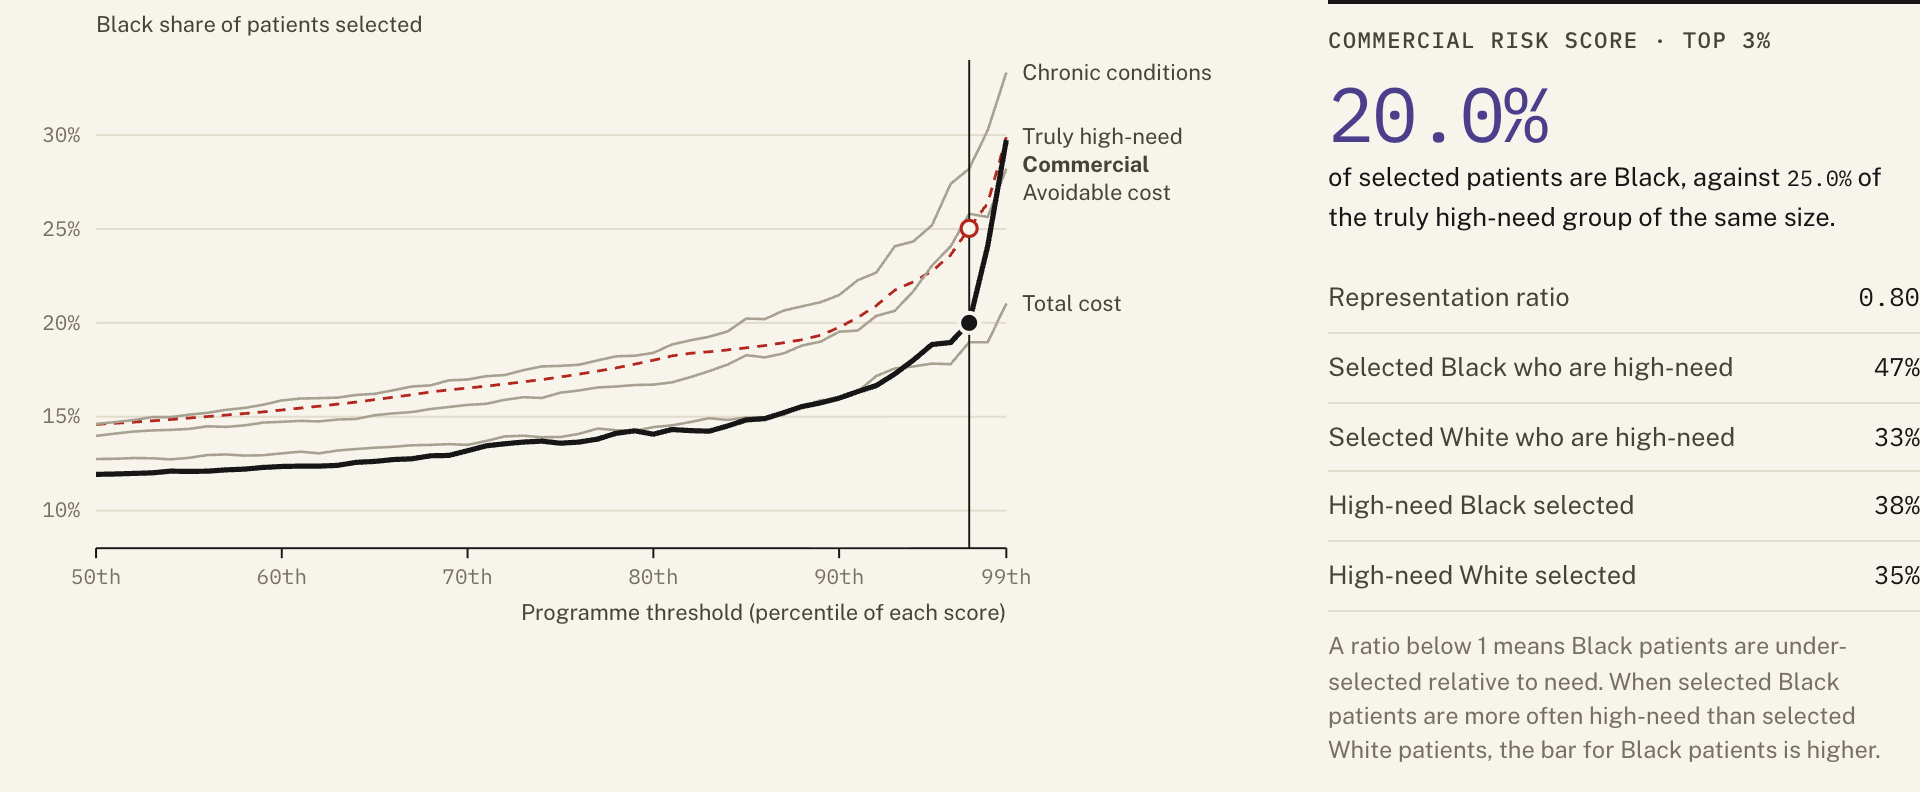
\includegraphics[width=0.495\textwidth]{figures/screens/explorer.png}}\hfill
\subfloat[Label mixer: blended-label frontier with live readout]{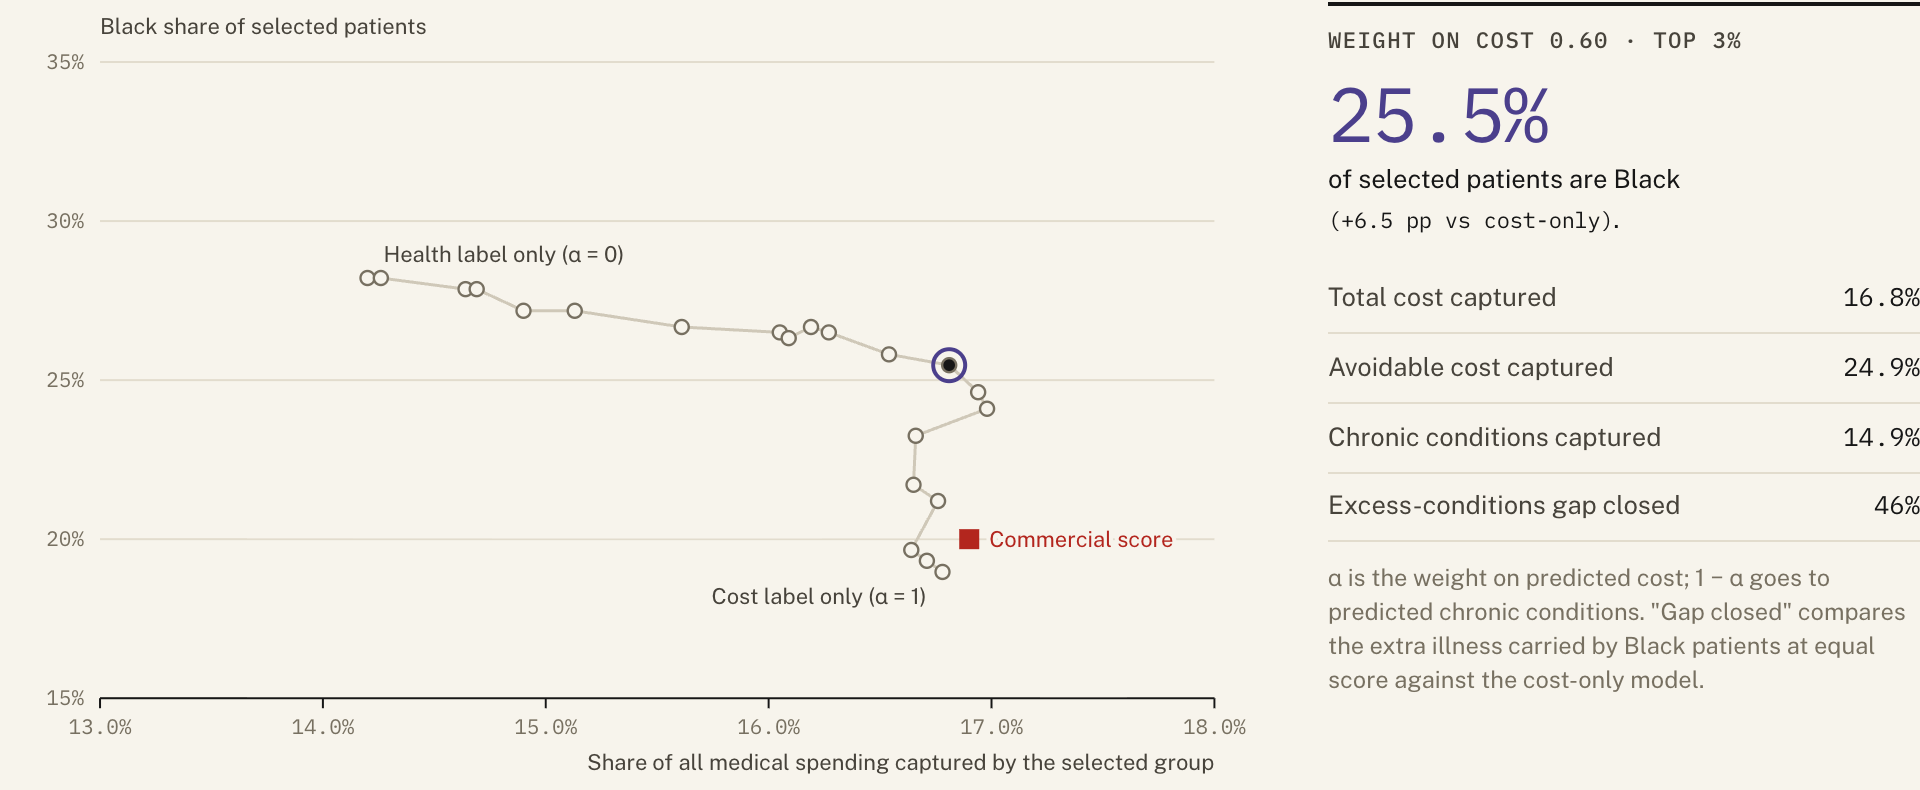
\includegraphics[width=0.495\textwidth]{figures/screens/mixer.png}}\\[1mm]
\subfloat[Regulatory matrix (October 2026 view); each cell opens its provision and sources]{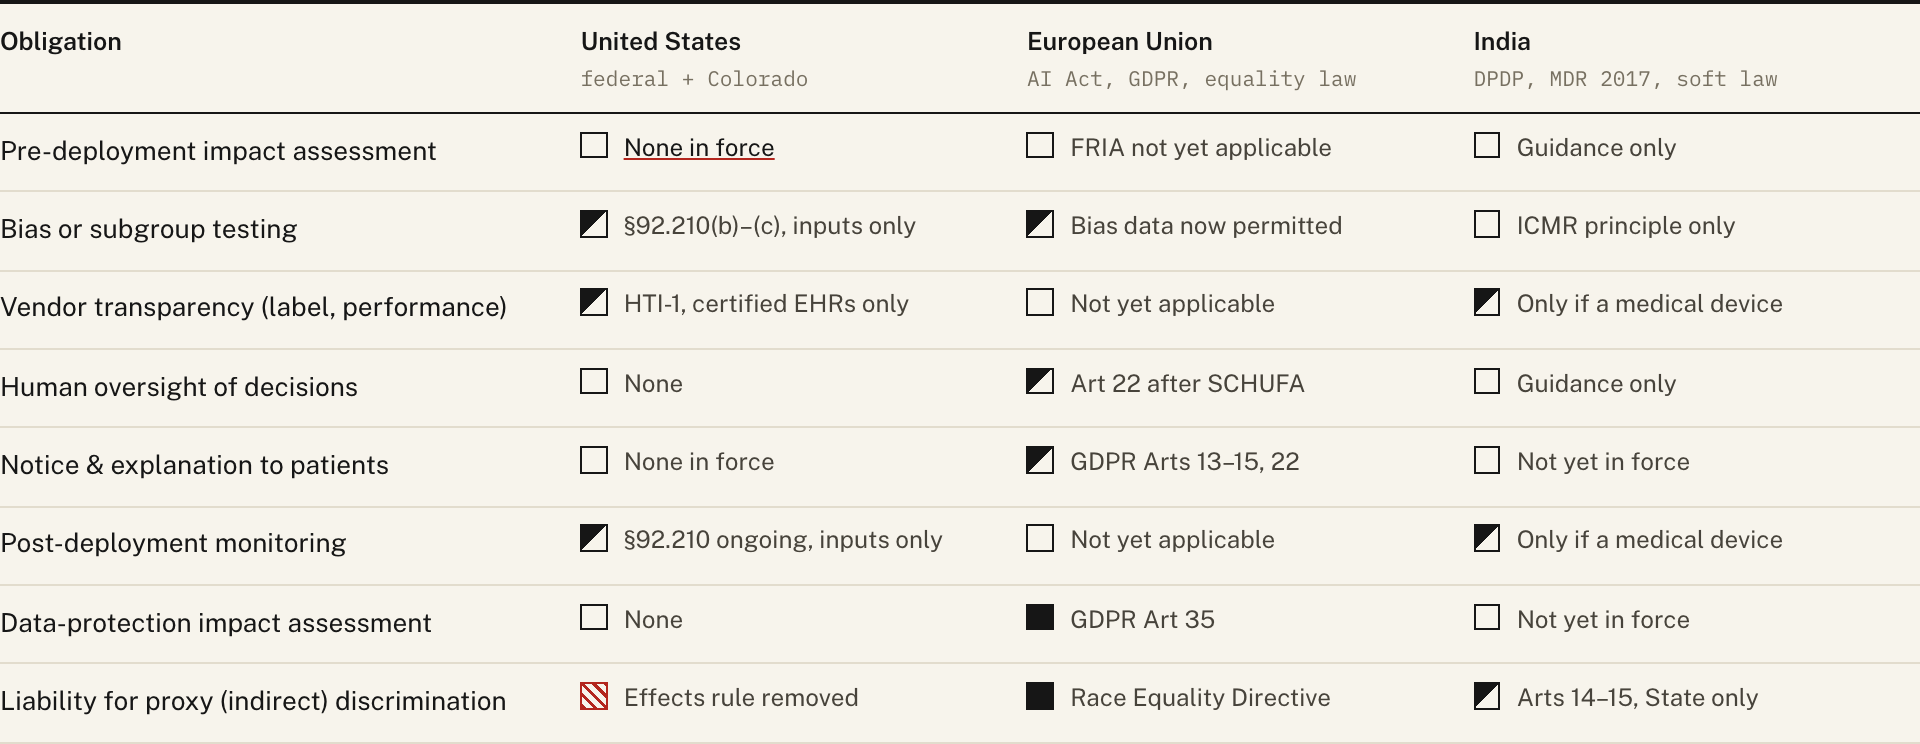
\includegraphics[width=\textwidth]{figures/screens/regulatory.png}}
\caption{Screenshots of the interactive dashboard (\site).}
\label{fig:screens}
\end{figure*}

\subsection{Replication fidelity}
Table~\ref{tab:fidelity} compares our synthetic-data results with the published real-data values. The direction and approximate size of every effect replicates. The swap reproduces the authors' published synthetic outputs exactly, both before and after the 2022 fix, and the label-choice shares match the authors' own synthetic results within 0.3 percentage points. Magnitudes differ from the real cohort (for example, a top-3\% Black share of \TopShareBlack{} against 17.7\%), as expected of synthetic data.

\begin{table}[t]
\centering
\caption{Replication fidelity: published values on the real cohort~\cite{obermeyer2019} and our values on the synthetic release~\cite{labsysmed}.}
\label{tab:fidelity}
\setlength{\tabcolsep}{4pt}
\begin{tabular}{@{}lrr@{}}
\toprule
Quantity & Published & This work \\
\midrule
Patient-years & 100,009 & 48,784 (synthetic) \\
Black share, $\geq$97th pct. & 17.7\% & 20.0\% \\
Conditions $\geq$97th, B vs W & 4.8 vs 3.8 & 6.6 vs 5.2 \\
Cost gap at equal health & $-$\$1{,}801 & $-$\$734 \\
Swap, original code & 17.7$\rightarrow$46.5\% & 18.4\%$\rightarrow$44.8\% \\
Swap, corrected code & $\rightarrow$59\% & $\rightarrow$59.2\% \\
Top 3\% Black, cost label & 14.1\% & 19.0\% \\
Top 3\% Black, avoidable cost & 21.0\% & 25.8\% \\
Top 3\% Black, conditions & 26.7\% & 28.2\% \\
\bottomrule
\end{tabular}
\end{table}


\subsection{The label, not the model}
Table~\ref{tab:labels} isolates the effect of the target variable. With identical features and estimator, the Black share of the top 3\% is \LabCost{} under the total-cost label, \LabAvoid{} under avoidable cost and \LabHealth{} under chronic conditions. The health label closes \ExcessHealth{} of the excess-conditions gap and the avoidable-cost label \ExcessAvoid. Each label performs best on its own outcome, so the choice is a value judgement about what the programme is for, not a technical detail.

\begin{table*}[t]
\centering
\caption{Label-choice experiment: composition and concentration of the top 3\% under each ranking (hold-out set, $n=\NHoldout$). ``Gap closed'' is the reduction in excess chronic conditions carried by Black patients at equal score, relative to the total-cost model.}
\label{tab:labels}
\begin{tabular}{@{}lrrrrrrr@{}}
\toprule
& \multicolumn{3}{c}{Black share of top 3\%} & \multicolumn{3}{c}{Share of outcome captured} & \\
\cmidrule(lr){2-4}\cmidrule(lr){5-7}
Ranking & Ours & 95\% CI & Published & Total cost & Avoid.\ cost & Conditions & Gap closed \\
\midrule
Commercial risk score & 20.0\% & 16.6\%--23.2\% & -- & 16.9\% & 22.7\% & 12.1\% & $-$4\% \\
Total cost & 19.0\% & 15.6\%--22.2\% & 14.1\% & 16.8\% & 22.9\% & 12.0\% & ref. \\
Avoidable cost & 25.8\% & 22.4\%--29.2\% & 21.0\% & 15.8\% & 26.4\% & 15.3\% & 53\% \\
Active chronic conditions & 28.2\% & 24.6\%--32.0\% & 26.7\% & 14.2\% & 23.8\% & 16.4\% & 94\% \\
\bottomrule
\end{tabular}
\end{table*}


\subsection{Mitigation is cheap}
Fig.~\ref{fig:frontier} traces the blended-label frontier. At $\alpha=0.6$, the top 3\% captures \BlendCost{} of total spending, the same as the cost-only model (\CostOnlyCost), while the Black share rises from \CostOnlyBlack{} to \BlendBlack{} and \BlendExcess{} of the excess-illness gap is closed. The trade-off a hospital might fear largely does not exist in this range. This is consistent with the vendor's own 84\% reduction using a combined label~\cite{obermeyer2019}.

\begin{figure}[t]
\centering
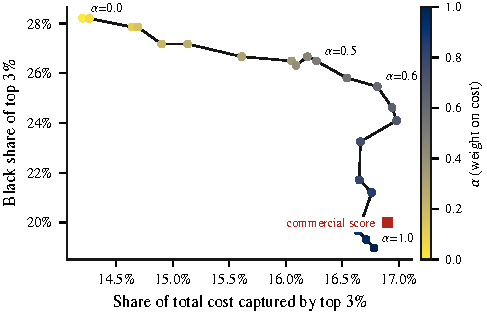
\includegraphics[width=\columnwidth]{figures/frontier.pdf}
\caption{Blended-label frontier at the top 3\%. Each point is a score $\alpha\,z(\hat{y}_{\text{cost}})+(1-\alpha)\,z(\hat{y}_{\text{health}})$; the square is the commercial score.}
\label{fig:frontier}
\end{figure}

\subsection{Selection fairness}
At the 97th percentile, the commercial score's representation ratio is \RepRatio: Black patients make up \LabCommercial{} of those selected but \NeedShare{} of the truly high-need (Table~\ref{tab:fairness}). The signature of a higher bar is in precision. \PpvB{} of selected Black patients are high-need against \PpvW{} of selected White patients, and this gap persists under both absolute definitions of need. Under the absolute definitions the representation ratio exceeds one, because those groups are larger and include many lower-scored patients. Representation is therefore definition-sensitive, while the precision gap is robust. With the health label, the precision gap disappears or reverses.

\begin{table}[t]
\centering
\caption{Selection fairness at the 97th percentile under three definitions of high need. Rep.\ ratio: Black share selected $\div$ Black share of high-need. PPV: share of selected patients who are high-need.}
\label{tab:fairness}
\setlength{\tabcolsep}{4pt}
\begin{tabular}{@{}lrrrr@{}}
\toprule
Ranking & Rep.\ ratio & PPV\textsubscript{B} & PPV\textsubscript{W} & TPR\textsubscript{B}/TPR\textsubscript{W} \\
\midrule
\multicolumn{5}{@{}l}{\textit{High need: Top 3\% by conditions}} \\
\quad Commercial & 0.80 & 47\% & 33\% & 1.07 \\
\quad Total cost & 0.76 & 51\% & 34\% & 1.05 \\
\quad Avoid.\ cost & 1.03 & 58\% & 54\% & 1.12 \\
\quad Conditions & 1.13 & 66\% & 69\% & 1.13 \\
\multicolumn{5}{@{}l}{\textit{High need: $\geq$3 conditions}} \\
\quad Commercial & 1.09 & 89\% & 73\% & 1.35 \\
\quad Total cost & 1.04 & 87\% & 71\% & 1.28 \\
\quad Avoid.\ cost & 1.41 & 91\% & 90\% & 1.58 \\
\quad Conditions & 1.54 & 93\% & 91\% & 1.79 \\
\multicolumn{5}{@{}l}{\textit{High need: HbA1c$\geq$9 or SBP$\geq$140}} \\
\quad Commercial & 1.21 & 36\% & 20\% & 2.23 \\
\quad Total cost & 1.15 & 41\% & 20\% & 2.39 \\
\quad Avoid.\ cost & 1.56 & 45\% & 27\% & 2.88 \\
\quad Conditions & 1.70 & 45\% & 28\% & 3.13 \\
\bottomrule
\end{tabular}
\end{table}


\subsection{Retrospective AIA}
Against the seven gates, the deployment \emph{failed} G1: in the selection band, Black patients carry about 1.4 more conditions (+\TopCondRel), far above the 0.25 tolerance. G2, G3, G5 and G6 were not performed. G0 and G4 were partial: the cost label was known but its mismatch with the programme's purpose was not flagged, and clinician review existed but did not correct the score. A single afternoon's analysis at G1 would have caught the bias before deployment.

\subsection{Regulatory review}
Table~\ref{tab:regulatory} summarises the coding.

\textbf{United States: no, and weaker than in 2019 on proxy discrimination.} The 2024 Section 1557 rule prohibits discrimination through patient-care decision-support tools (45~CFR~92.210(a)). Its duty to identify and mitigate risk, in force since 1~May 2025, applies only to tools whose \emph{input variables} measure race, colour, national origin, sex, age or disability~\cite{hhs1557,ocr2025}, so a race-blind cost model does not trigger it. HTI-1 source attributes bind only certified health-IT developers~\cite{hti1}, and the HTI-5 proposal would remove them~\cite{hti5}. FDA's January 2026 CDS guidance is silent on population risk scores~\cite{fda_cds}. Colorado's 2024 AI Act, the only US law requiring deployer impact assessments, was replaced in May 2026 by a notice-based statute effective 2027 whose enforcement is stayed~\cite{colorado}. EO~14281 directed agencies to deprioritise disparate-impact enforcement, and HHS removed the effects provision from its Title VI regulations effective 24~July 2026~\cite{eo14281,hhs_tvi2026}. In 2019 that provision was the federal route for challenging a facially neutral criterion with discriminatory effects, enforceable by the agency though not by private suit~\cite{sandoval2001}. Our reading is that this route has narrowed. The Algorithmic Accountability Act remains unenacted~\cite{aaa2025}.

\textbf{European Union: partly.} A GDPR data-protection impact assessment was already mandatory in 2019 for large-scale health-data processing (Art.~35(3)(b)), and the Race Equality Directive prohibits unjustified indirect discrimination in healthcare~\cite{gdpr,red2000}. These are the only full marks in the table. After SCHUFA~\cite{schufa2023}, a score that decisively drives enrolment may also engage Art.~22. The AI Act's bias examination (Art.~10), deployer duties (Art.~26) and fundamental-rights impact assessment (Art.~27) are the closest match to our AIA. However, the Digital Omnibus moved Annex~III obligations to 2~December 2027~\cite{omnibus2026}, and Annex~III 5(a) covers eligibility decisions taken by or on behalf of \emph{public authorities}, so a private hospital is probably outside it~\cite{euaiact}. The new Art.~4a permits processing ethnicity data for bias detection but does not require it.

\textbf{India: not yet.} India has the richest set of voluntary principles~\cite{icmr2023,niti2021,meity2025} and the fewest binding duties. The DPDP Act's main obligations begin around 13~May 2027, and Rule~13's annual DPIA and check that ``algorithmic software'' does not endanger data principals' rights apply only to designated Significant Data Fiduciaries~\cite{dpdp2023,dpdprules2025}. CDSCO's July 2026 software guidance applies only if the tool is a medical device~\cite{cdsco2026}. Articles 14--15 bind the State, so public schemes are covered but private hospitals largely are not. In India, the same proxy would track caste, gender, rurality and income rather than race, because claims-based utilisation reflects those access gaps.

\begin{table*}[t]
\centering
\caption{Would the law require it? Obligations applicable to a hospital deploying a race-blind, cost-trained enrolment score, coded for October 2019, October 2026 and as scheduled for December 2027. \mY\ binding and applies; \mP\ binding but narrow, not triggered, or adopted but not yet applicable; \mN\ no binding duty (soft law noted in text); \mX\ protection removed since 2019. Status as of 7 October 2026.}
\label{tab:regulatory}
\setlength{\tabcolsep}{5pt}
\begin{tabular}{@{}l ccc ccc ccc@{}}
\toprule
& \multicolumn{3}{c}{United States} & \multicolumn{3}{c}{European Union} & \multicolumn{3}{c}{India} \\
\cmidrule(lr){2-4}\cmidrule(lr){5-7}\cmidrule(lr){8-10}
Obligation & 2019 & 2026 & 2027 & 2019 & 2026 & 2027 & 2019 & 2026 & 2027 \\
\midrule
Pre-deployment impact assessment & \mN & \mN & \mN & \mN & \mN & \mP & \mN & \mN & \mN \\
Bias or subgroup testing & \mN & \mP & \mP & \mN & \mP & \mP & \mN & \mN & \mP \\
Vendor transparency (label, performance) & \mN & \mP & \mP & \mN & \mN & \mP & \mN & \mP & \mP \\
Human oversight of decisions & \mN & \mN & \mN & \mP & \mP & \mP & \mN & \mN & \mN \\
Notice \& explanation to patients & \mN & \mN & \mP & \mP & \mP & \mP & \mN & \mN & \mP \\
Post-deployment monitoring & \mN & \mP & \mP & \mN & \mN & \mP & \mN & \mP & \mP \\
Data-protection impact assessment & \mN & \mN & \mN & \mY & \mY & \mY & \mN & \mN & \mP \\
Liability for proxy (indirect) discrimination & \mP & \mX & \mX & \mY & \mY & \mY & \mP & \mP & \mP \\
\bottomrule
\end{tabular}
\end{table*}


\subsection{Dashboard}
Fig.~\ref{fig:screens} shows the dashboard. Readers can switch the calibration chart between health and cost, move the programme threshold, change the blended label, step the regulatory matrix between 2019, 2026 and 2027, and open the citation behind any cell.



\subsection{Summary of findings}
\begin{enumerate}
\item The bias replicates, and the corrected counterfactual (\SwapFixed) is starker than the published one.
\item The label, not the model, drives the disparity; a health label closes \ExcessHealth{} of the excess-illness gap.
\item A blended label recovers much of the gap at no loss in cost captured.
\item Human review did not correct the score.
\item A label-validity gate would have caught the problem before deployment.
\item Seven years on, no jurisdiction clearly mandates that gate for this deployment. The EU comes closest; US federal protection has narrowed; India relies on soft law until 2027.
\end{enumerate}

%=====================================================================
\section{Conclusion}
%=====================================================================
Detection was never the hard part. The bias in cost-as-proxy risk scores can be found with data every deploying hospital already holds, and it can be largely fixed by changing the label. What was missing in 2019 was an obligation for anyone to look. We answer the four questions posed in Section~I. \emph{Who is responsible?} The vendor is responsible for the label; the deploying hospital, and a payer that mandates the tool, are accountable for its use. \emph{What assessment should have been required?} A Level III--IV impact assessment built around a label-validity test. \emph{Would the law now mandate it?} In the US, no; the relevant protections are keyed to inputs rather than labels and have narrowed since 2019. In the EU, partly; a DPIA and equality law apply now, and AI-specific duties arrive in December 2027, probably only for public bodies. In India, not yet; binding duties begin in 2027, and then only for designated fiduciaries.

\textbf{Limitations.} The cohort is synthetic and has no patient identifiers, so intervals treat patient-years as independent. Chronic-condition counts are themselves shaped by access to care. ``White'' denotes all non-Black patients in the source data. The regulatory coding is our reading as of 7~October 2026, not legal advice, and several instruments (HTI-5, Colorado's litigation, the GDPR omnibus) were still in motion. Future work could extend the audit to Indian claims data along caste, gender and rural axes, and test the G1--G2 thresholds against clinical outcomes.

\section*{Data and Code Availability}
Code, generated data, figures and this paper's source: \repo. Interactive dashboard: \site. The synthetic cohort is available from its authors~\cite{labsysmed}.

\IEEEtriggeratref{33}
\bibliographystyle{IEEEtran}
\bibliography{refs}

\end{document}
